\chapter{Образование нано- и микромасштабных частиц при хрупком разрушении горных пород} \label{chapt3}

Рассмотрены особенности образования мелкодисперсных частиц при разрушении гранитного образца изгибом, разрывом, сдвигом и кручением. Обнаружено образование нано- и микромасштабных частиц с размерами от 100 нм до 1 мм. Распределение частиц хорошо совпадает с распределением Розина-Раммлера.

Большая роль нано- и микромасштабных частиц в среде обитания по-новому затрагивает вопрос о достижении теоретического предела прочности частиц при уменьшении их размера, так как количество и размерно-массовое соотношения частиц после измельчения определяются такими свойствами исходного материала как прочность. Фактический предел прочности — нагрузка, при которой происходит хрупкое разрушение материала — заметно отличается от теоретически рассчитанного из параметров кристаллической решетки значения, иногда разница соответствует нескольким порядкам величины. Такое поведение прочности связывают с наличием различных нарушений упорядоченной кристаллической структуры вещества —  микротрещин и дислокаций,— которые выступают в роли концентраторов напряжений, увеличивая напряжение его на своих границах в сотни раз, и, реализуя локально теоретическую критическую нагрузку. Широкий разброс прочности для одного минерала или горной породы как раз и можно объяснить индивидуальным набором дефектов для каждого образца.
Таким образом, с уменьшением размера частицы, вероятность наличия дефектов кристаллической структуры уменьшается, следовательно, можно ожидать увеличения её прочности. 
Классическими стали опыты Гриффитса по вытягиванию тонких стеклянных волокон в 20-х – 30-х годах. Чем тоньше были полученные нити, тем они оказывались прочнее. Сначала их прочность увеличивалась медленно, но по мере того, как они становились очень тонкими, прочность возрастала весьма быстро. Прочность волокон диаметром около 2,5 мкм сразу после вытягивания составляла 600 кг/мм2 и более, а спустя несколько часов падала примерно до 350 кг/мм2. Кривая зависимости прочности от диаметра волокна росла столь стремительно, что трудно было установить верхний (максимальный) предел для величины прочности.

Гриффитс не мог ни изготовить, ни испытать волокна тоньше примерно 2,5 мкм. Однако он экстраполировал кривую "прочность-размер" в область ничтожно малых толщин, и оказалось, что прочность тончайших нитей должна быть около 1100 кг/мм2. Вычисленная величина прочности для его стекла была чуть меньше 1400 кг/мм2. Поэтому Гриффитс сделал вывод, что ему практически удалось приблизиться к теоретической прочности, и, если бы на самом деле можно было сделать более тонкие волокна, их прочность была бы очень близка к теоретической.

Также известны опыты А. Ф. Иоффе по разрыву кристаллов каменной соли, в которых показано влияние состояния поверхности образца (наличие трещинок, царапин), а также среда, в которой он находится, на прочность. А. Ф. Иоффе измерял прочность кристаллов каменной соли на воздухе и при погружении в воду, и оказалось, что она увеличивается с 0,5 до 160 кг/мм2. Такое изменение можно объяснить растворением в воде приповерхностного слоя кристаллов и ликвидацией дефектов этого слоя.

В целом, как отмечал Гриффитс, дефекты на поверхности образца играют более важную роль в разрушении образца, чем внутренние.

Ряд других работ также затрагивает вопрос достижения теоретической прочности. Например, в работе М. И. Койфмана [Койфман М. И., 1943] исследуется прочность кварца, корунда, искусственного корунда и карбида кремния в зависимости от размеров зерен, и устанавливается постепенное увеличение прочности при уменьшении размеров зерен. Минимальный размер зерен в опытах составил 90 мкм, что для карбида кремния дало увеличение прочности в 10 раз.

Современные упоминания предела прочности связаны с получением идеальных наномасштабных структур из атомов кремния со свойствами, которые нельзя назвать ни хрупкими, ни пластичными [Esser M., 2008]. Такие образцы, так как есть ещё дополнительная возможность определять их форму, обнаруживают очень высокие прочностные характеристики.
Исследования распределений нано- и микромасштабных частиц, образованных при проведении массовых взрывов на карьерах, а также частиц полученных после проведения многократных химических взрывов [Дубовской А.Н., Перник Л.М., Попель С.И., 2008], дают основания предполагать, что предполагаемое изменение прочности частиц при уменьшении их размера не проявляется — измеренные распределения согласуются с теоретическими Розина-Раммлера и Колмогорова.  Однако, ввиду высокой энергоёмкости взрыва на единицу породы, можно предположить, что напряжение ударной волны достаточно высоко и сравнимо по величине с теоретическим пределом прочности.

Таким образом, проведение эксперимента по изучению предела прочности, но с использованием только малых напряжений (существенно меньших теоретического предела прочности) при разрушении горной породы, поможет уточнить вывод и [Дубовской А.Н., Перник Л.М., Попель С.И., 2008].


\section{Эксперименты по хрупкому разрушению горной породы} \label{sect4_1}

Для исследования возможности образования наночастиц при разрушении скальной породы были проведены следующие эксперименты. 

Образец скальной породы (серый гранит) размером 20х40х60 мм посередине ослаблялся надпилом для фиксации места разрушения. 

      На рисунке~\ref{img:4scheme} показана схема опыта при разрушении образца на излом. Образец помещался на П-образную пресс-форму на дне которой находился проводящий скотч для сбора пыли, пригодный для дальнейшего анализа на электронном микроскопе. Разрушение образца производилось с помощью школьного пресса.
	  
	  \begin{figure} [h] 
	    \center
	    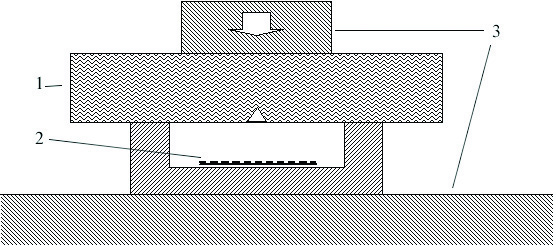
\includegraphics[width=120mm]{pic41}
	    \caption{Схема проведения опыта по излому гранитного образца на прессе. 1 – гранитный образец; 2 – скотч для фиксации частиц;  3 – элементы пресса.} 
	    \label{img:4scheme}  
	  \end{figure}
	  
      Аналогичным образом был проведен опыт для разрушения образца на сдвиг. При этом части образца зажимались в специальные металлические обоймы, которые затем с помощью пресса сдвигались относительно друг друга.
	  
     В опытах при разрушении на кручение и разрыв использовался токарный станок. Образец одним концом зажимался в шпиндель, а другим в заднюю бабку станка. Разрушение образца достигалось соответственно при вращении шпинделя или сдвиге задней бабки.
	 
Полученные подложки с частицами, выделенными после разрушения палочки, были проанализированы с помощью электронного микроскопа по методике описанной в [Дубовской А.Н., Перник Л.М., Попель С.И., 2008].


\section{Результаты} \label{sect4_2}

В ходе обработки экспериментальных данных были обнаружены наночастицы с минимальными размерами от 100 до 160 нм. Для всех четырех опытов очевидного различия нижней границы размеров частиц не было отмечено.  

На рисунке~\ref{img:4rr} показаны результаты гранулометрического анализа для выполненных экспериментов в координатах Розина-Раммлера.  

	  \begin{figure} [h] 
	    \center
	    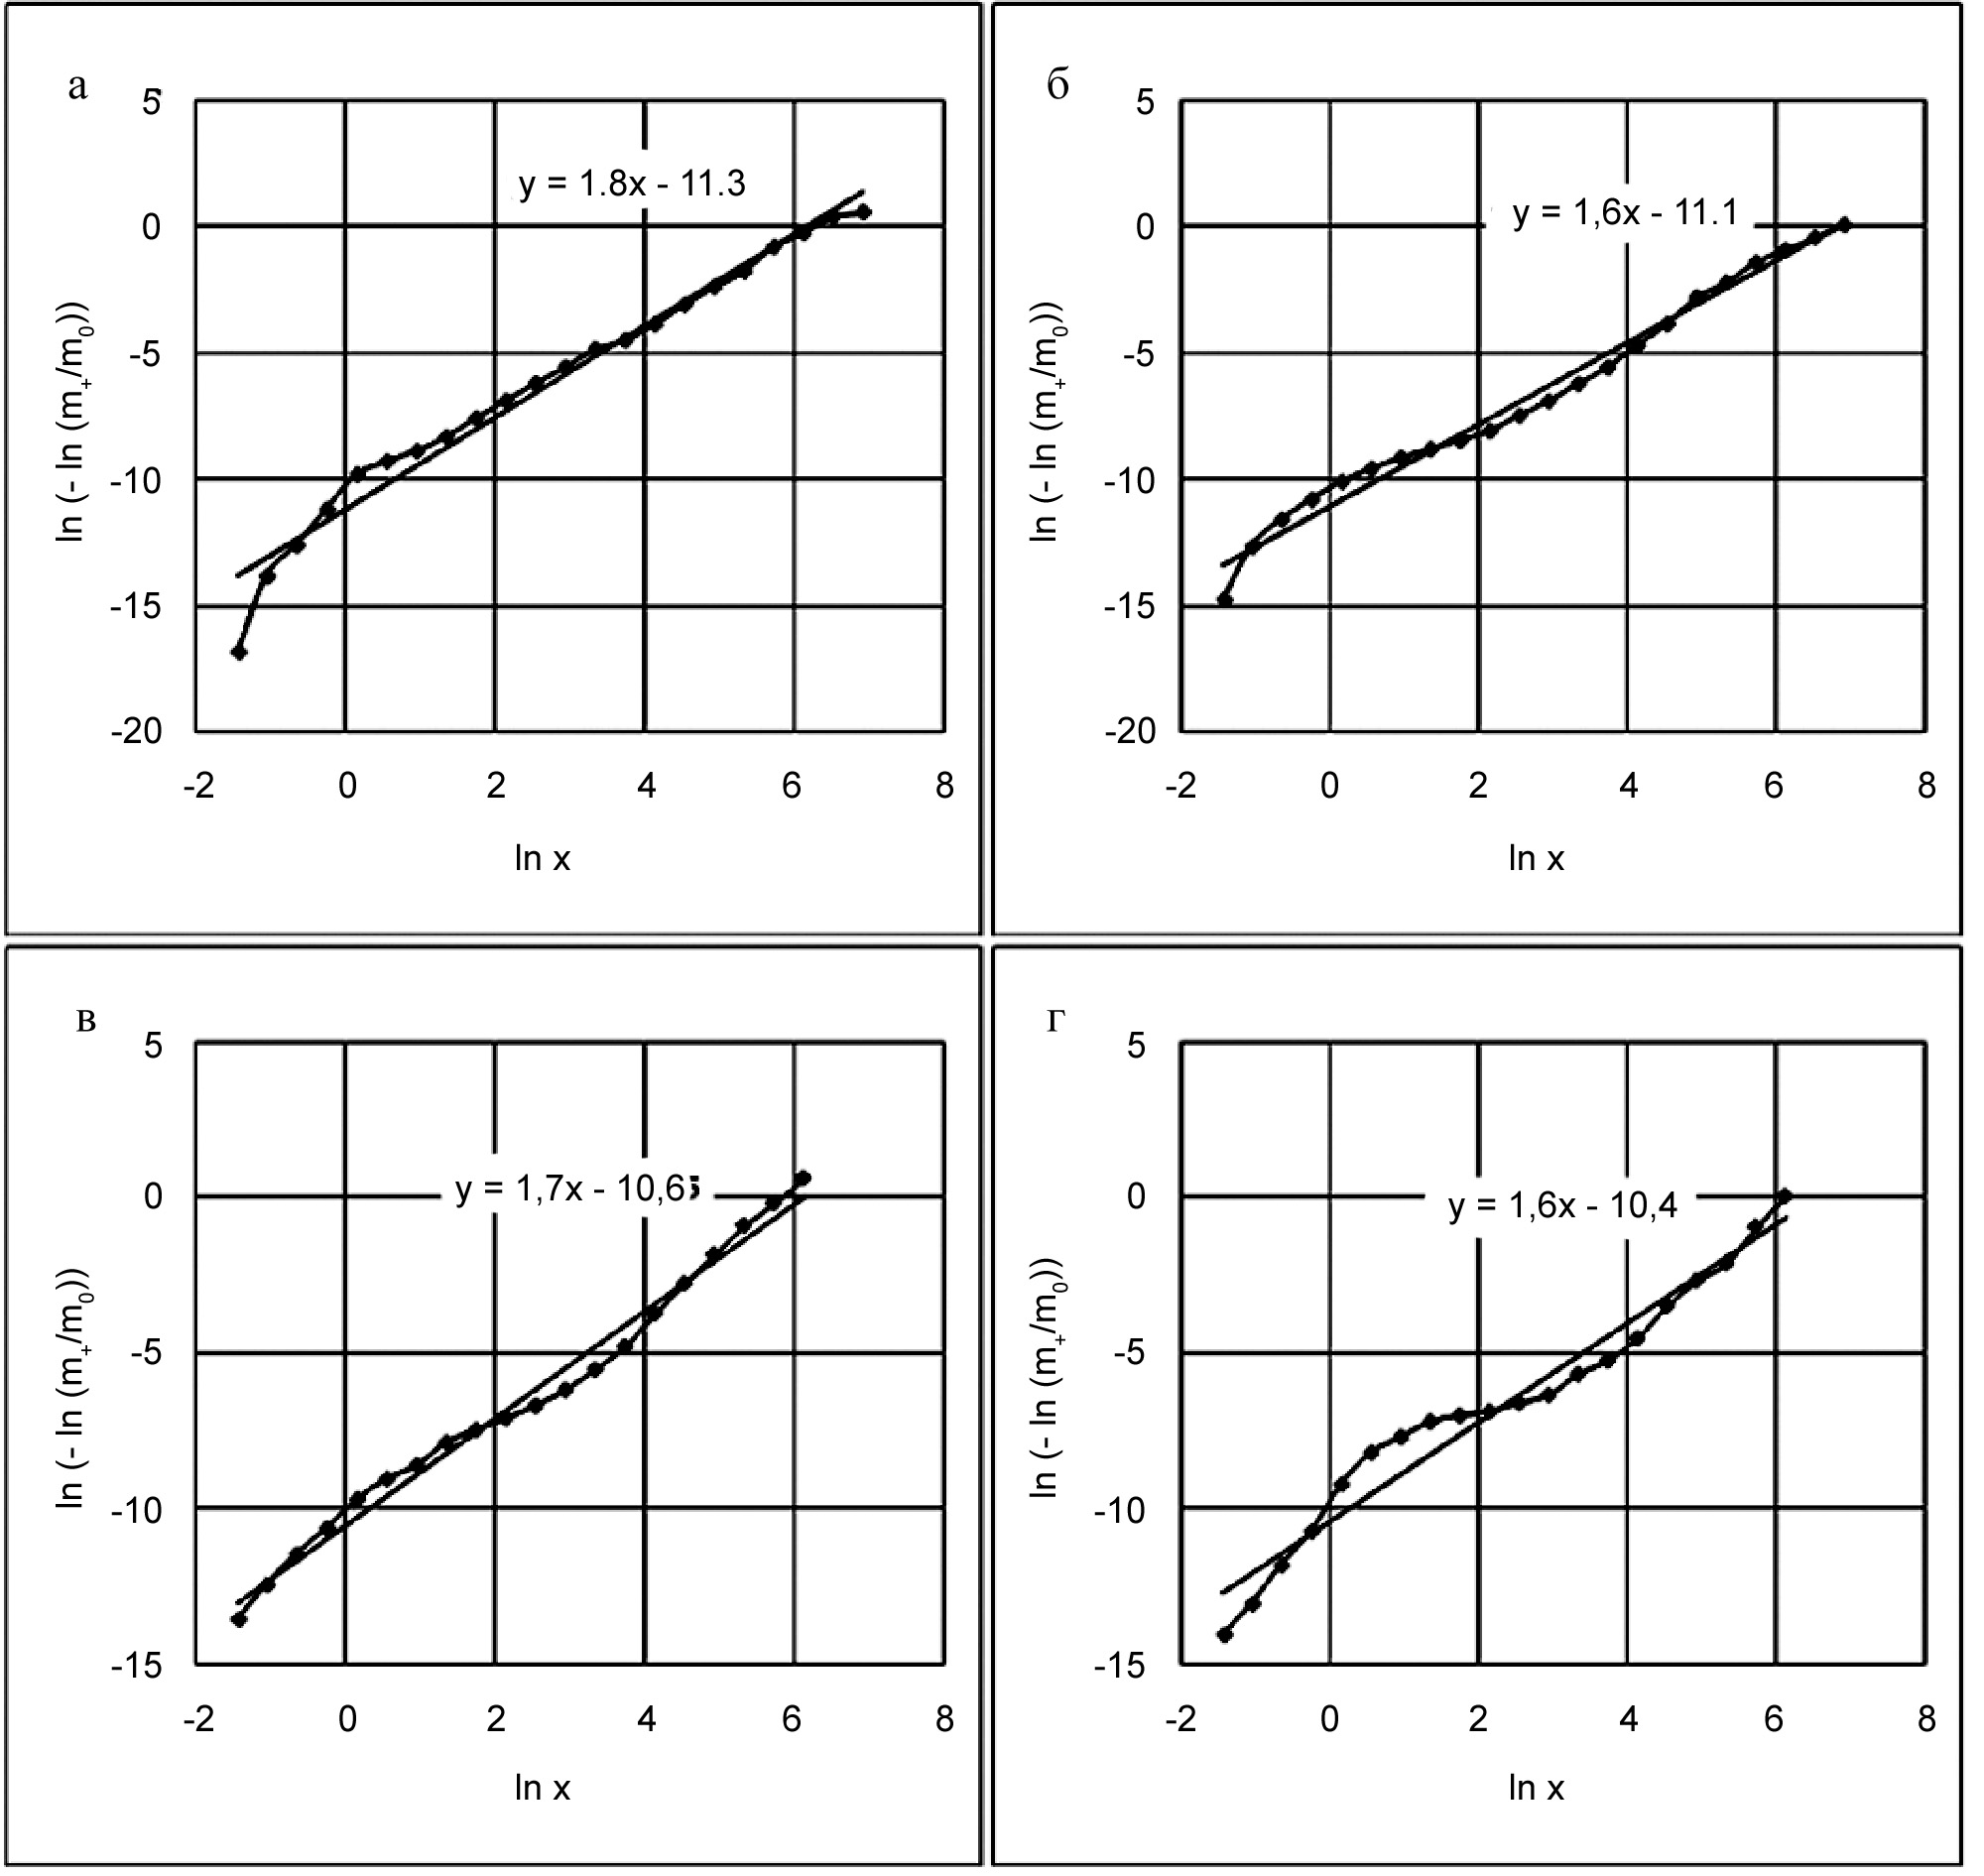
\includegraphics[width=120mm]{pic42}
	    \caption{Гранулометрический состав частиц, образованных в результате экспериментов, по изгибу (а), сдвигу (б), кручению (в) и разрыву (г) гранитного образца (в координатах Розина-Раммлера).} 
	    \label{img:4rr}  
	  \end{figure}
	  
Видно, что в данных координатах, зависимость близка к прямой линии. Наиболее сильное отклонение от прямой отмечается для самых малых размеров наночастиц, что может быть связано, как с потерей самых мелких частиц при экспериментах, так и приближение к теоретической прочности испытываемого материала.
Таким образом, в экспериментах по разрушению горных пород относительно малыми (по сравнению с проведенными взрывными экспериментами [Дубовской А.Н., Перник Л.М., Попель С.И., 2008]) энергетическими затратами, было зарегистрировано наличие наночастиц. Это может быть связано как с образованием этих частиц при разрушении горной породы, так и с наличием свободных наночастиц в исходных образцах.






\clearpage